\documentclass[conference]{IEEEtran}
\IEEEoverridecommandlockouts
% The preceding line is only needed to identify funding in the first footnote. If that is unneeded, please comment it out.
\usepackage{cite}
\usepackage{amsmath,amssymb,amsfonts}
\usepackage{algorithmic}
\usepackage{graphicx}
\usepackage{textcomp}
\usepackage{xcolor}
\usepackage{hyperref}
\usepackage{float}


\def\BibTeX{{\rm B\kern-.05em{\sc i\kern-.025em b}\kern-.08em
    T\kern-.1667em\lower.7ex\hbox{E}\kern-.125emX}}
\begin{document}

\title{Building a Small Language Model \\ Configuration, Training, Inference}

\author{\IEEEauthorblockN{Samrat Kar}
Bangalore, India}

\maketitle

\begin{abstract}
This paper develops a small language model (SLM). Trains it with the Julius Caesar text. And then it uses the it generates new texts based on the knowledge gained form the text. The model parameters are stored for future use and application development. The various fine tuning is done, to improvise the model to reduce overfitting. 
\end{abstract}

\section{Introduction}
The code implements the multi-head attention mechanism using Transformer architecture. The Julius Caesar text is taken from Project Gutenberg and it is used to train the model. 

\section{Steps to build the SLM}
\begin{itemize}
    \item Get the dataset and 
    \item Tokenize the dataset using tiktoken library.
    \item Split the data set into test and train and store the data set in a memory-mapped array to avoid RAM overload.
    \item Create input-output batches for the dataset for both test and train split.
    \item Do the layer normalization for regularization
    \item Compute \textbf{Context Matrix} 
    \begin{itemize}
        \item Compute \textbf{Causal Attention Score} Matrix (MHA: Multi-head attention)
        \begin{itemize}
            \item initialize the $W_q, W_k, W_v$ matrix
            \item Query Matrix $Q = X \times W_q$ (X = input matrix)
            \item Key Matrix $K =  X \times W_k$ 
            \item Value Matrix $V = X \times W_v$
            \item Attention score $att = (Q \times K^T)/ \sqrt{dim}$
            \item Masking attention score by $-\infty$ on the upper diagonal of the Attention Score.
            \item $att = softmax(att \ score)$
            \item self attention dropout
        \end{itemize}
        \item \textbf{Context Matrix} = $y = att \times V$
    \end{itemize}
    \item Dropout on \textbf{Context matrix} 
    \item Pass context matrix to \textbf{Multi-layer perceptron feedforward neural network. (MLH)} with GELU activation function to train the model
\end{itemize}

\section{Codebase}
\href{https://colab.research.google.com/github/samratkar/samratkar.github.io/blob/main/_posts/concepts/genai/notes-codes/slm-from-scratch/slm-jc.ipynb}{Working SLM codebase}

\section{Baselined Model Config}
learning rate = 1e-4 \\
max iters = 10000 \\
warmup steps = 2000 \\
min lr = 5e-4 \\
eval iters = 500 \\
batch size = 8 \\
block size = 128 \\
vocab size=50257 \\
block size=128 \\
number of layers=4 \\
number of heads=4 \\
embedding dimension=768 \\
dropout=0.01 \\
bias=True 

\section{Dataset}
\href{https://www.gutenberg.org/cache/epub/1522/pg1522.txt}{Julius Caesar full text}

\section{epochs : 500}

\begin{figure}[H]
    \centering
    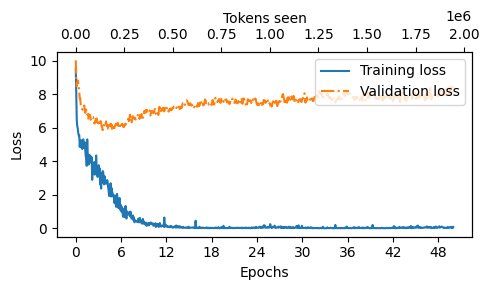
\includegraphics[width=0.5\linewidth]{training-validation-loss.png}
    \caption{Trg, Test Loss}
    \label{fig:epoch500}
\end{figure}

\section{epochs : 4000}
\begin{figure}[H]
    \centering
    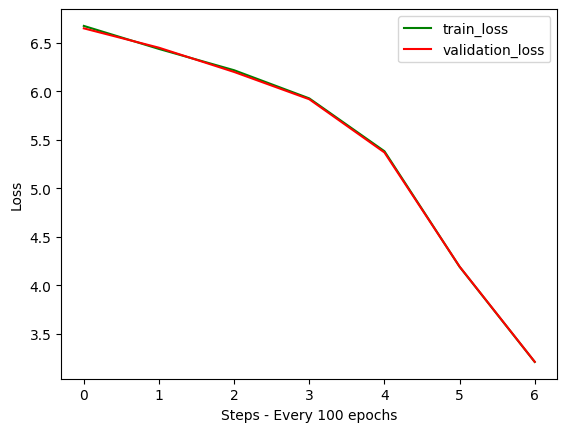
\includegraphics[width=0.5\linewidth]{4kep.png}
    \caption{Trg, Test Loss}
    \label{fig:epoch4000}
\end{figure}

\section{epochs : 10,000}
\begin{figure}[H]
    \centering
    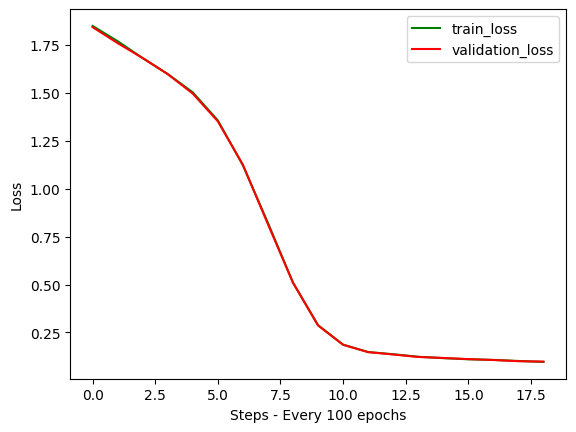
\includegraphics[width=0.5\linewidth]{10kep.png}
    \caption{Trg, Test Loss}
    \label{fig:epoch10000}
\end{figure}

\section{epochs : 20,000}
\begin{figure}[H]
    \centering
    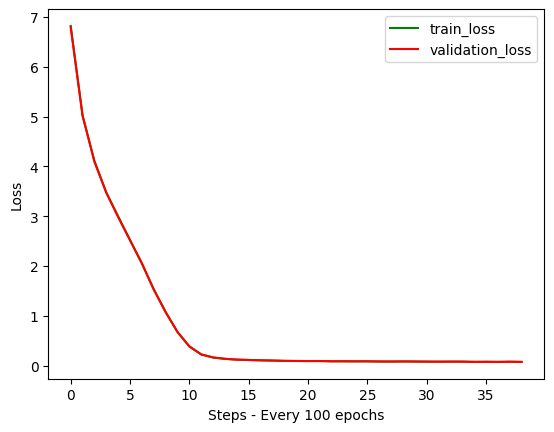
\includegraphics[width=0.5\linewidth]{20Kep.png}
    \caption{Trg, Test Loss}
    \label{fig:epoch20000}
\end{figure}

\end{document}
